\documentclass[12pt,a4paper]{report}

%Allgemeine Dokumenteigenschaften
\usepackage[top=3cm,left=4cm, bottom=3cm, right=2cm]{geometry}
\usepackage[onehalfspacing]{setspace}

%Einstllunge für die Text- und Spracheigenschaften
\usepackage[T1]{fontenc}
\usepackage[utf8x]{inputenc}
\usepackage[ngerman]{babel}
\usepackage{helvet}
\renewcommand{\familydefault}{\sfdefault}

\usepackage{chemfig}
\usepackage{mhchem}


\usepackage{amssymb}
\usepackage{amsmath}
\usepackage{booktabs}

\usepackage{upgreek}
\usepackage{textcomp}


\usepackage{hyperref}
\usepackage{blindtext}

\usepackage{titlesec}
\titlespacing{\chapter}{0pt}{-25pt}{10pt}
\titleformat{\chapter}{\LARGE\bfseries}{\thechapter\ }{0.1em}{}
\titleformat{\section}{\Large\bfseries}{\thesection\ }{0.1em}{}
\titleformat{\subsection}{\large\bfseries}{\thesubsection\ }{0.1em}{}
\begin{document}
	\tableofcontents
	\chapter{Zusammenfassung}
	\chapter{Einleitung}
	Metal ions play essential roles in countless biological processes
	and consequently are key to many aspects of medicine.
	However, if a metal ion is out of context, present at abnormally
	high concentrations, or intrinsically toxic, then detrimental
	impacts on the environment and human health become key.
	Consequently, the selective and sensitive detection of hard and/
	or soft metal ions is essential in a multitude of scenarios. To meet
	this challenge, finely tuned calixarene fluorescent probes with both suitable ligating sites (O, N, and S) and attendant fluorophores have been developed. \\
	\ \\
	Zn2+ is an important
	micronutrient in humans, deficiency of which may cause severe
	metabolic and developmental detriments.88 The concentration
	of Zn2+ in blood serum is approximately 19 μM, and deviation
	from this concentration is associated with various disorders,
	including Alzheimer’s disease, hyperalgesia, and diabetes.\\
	\ \\
	https://sci-hub.hkvisa.net/10.1021/acs.chemrev.8b00605
	\chapter{Theorie}
	\section{Lab-on-a-chip}
	\section{Photoinduzierter Elektronentransfer (PET)}
	\section{Fluoreszenzsensoren}
	\section{Calixarene}
	\chapter{Problemstellung}
	\chapter{Ergebnisse}
	\section{Spektroskopische Charakterisierung}
	\subsection{Pyranin}
	Es wurde ein UV/Vis-Absorptionsspektrum von Pyranin in Wasser in einem Wellenlängenbereich von 300 - 480 nm aufgenommen. Die spektroskopischen Charakteristika können \textbf{\autoref{tab:UVVisPyranin}} entnommen werden. 
	\begin{table}[h!]
		\centering
		\textbf{\caption{\textnormal{Spektroskopische Merkmale des Pyranins in Wasser.}}}
		\label{tab:UVVisPyranin}
		\begin{tabular}{p{2.5cm}p{2.5cm}l}
			\toprule
			Peak&$\mathbf{\uplambda_{max}}$/nm &\ce{A_{max}} \\ 
			\hline
			2&370&0,048\\
			3&404&0,058\\
			\bottomrule
		\end{tabular}
	\end{table}\\
	Das Absorptionsspektrum ist durch zwei Banden charakterisiert, welche sich im UB-B (370 nm) und dem violetten Bereich des sichtbaren Lichtes (404 nm). Letztere sorgt für die intensive gelbe Farbe des Pyranins.
		\begin{figure}[h!]
			\centering
			\includegraphics*[width=0.8\textwidth]{UVVisPyranin.jpg}
			\textbf{\caption{\textnormal{UV/Vis-Absorptionsspektrum des Pyranins in Ethanol im Wellenlängenbereich von 250-480 nm.}}}
			\label{fig:UVVisPyranin}
		\end{figure}\\
	Die Lage der Absorptionsbanden ist stark vom pH-Wert des Lösungsmittels abhängig (pKs = 7,4). Der Effekt ist auf die Deprotonierung der Hydroxygruppe (\textbf{\autoref{fig:StrukturPyranin}}) und der sich daraus ergebenden Erhöhung des +M-Effekts zurückzuführen, welcher einen zunehmend bathochromen Shift der Peaks verursacht. Die deprotonierte Pyraninspezies ist an einem Absorptionsmaximum bei 460 nm erkennbar. Der Vergleich mit dem gemessenen Absorptionsspektrum zeigt, dass es sich im Experiment erwartungsgemäß um die protonierte Form des Pyranins handelt. 
		\begin{figure}[h!]
			\centering
			\includegraphics*[width=0.5\textwidth]{StrukturPyranin.png}
			\textbf{\caption{\textnormal{Das Grundgerüst des Fluoreszenzfarbstoffs Pyranin (8-Hydroxy-1,3,6- pyrentrisulfonsäuretrinatriumsalz) basiert auf Pyren. Der bathochrome Effekt der OH-Gruppe wird durch deren Deprotonierung verstärkt.}}}
			\label{fig:StrukturPyranin}
		\end{figure}\\
	\ \\
	Zur Zuordnung der Übergänge existieren verschiedene Modelle
	Es wurde ein Fluoreszenzspektrum des Pyranins bei einer Anregungswellenlänge von $\mathbf{\lambda}$\textbf{\ce{_{exc}}} = 420 nm in Ethanol aufgenommen (\textbf{\autoref{fig:FluoreszenzPyranin}}). Das Emissionsmaximum liegt bei 504 nm und wird von der Literatur bestätigt. Der, verglichen mit dem Absorptionsspektrum, bathochrome Shift des Emissionspeaks ist auf die typisch positive Solvatochromie des Pyranins zurückzuführen. Die Fluoreszenzlebensdauer (\textbf{\autoref{fig:FLDPyranin}}) liegt bei 1,14 s. 
		\begin{figure}[h!]
			\centering
			\includegraphics*[width=0.8\textwidth]{FluoreszenzPyranin.jpg}
			\textbf{\caption{\textnormal{Fluoreszenzspektrum des Pyranins in Ethanol bei einer Anregungswellenlänge von 420 nm.}}}
			\label{fig:FluoreszenzPyranin}
		\end{figure}
		\begin{figure}[h!]
			\centering
			\includegraphics*[width=0.8\textwidth]{FluoreszenzPyranin.jpg}
			\textbf{\caption{\textnormal{Fluoreszenzspektrum des Pyranins in Ethanol bei einer Anregungswellenlänge von 420 nm.}}}
			\label{fig:FLDPyranin}
		\end{figure}\\
	\newpage 
	\subsection{Ligand und Komplex}
	Es wurde ein UV/Vis-Absorptionsspektrum des reinen Liganden sowie des Liganden unter Zugabe von Zinkacetat aufgenommen (\textbf{\autoref{fig:UVVISLigandKomplex}}). Die spektroskopischen Merkmale sind \textbf{\autoref{tab:UVVisLigandKomplex}} zu entnehmen.
		\begin{table}[h!]
			\centering
			\textbf{\caption{\textnormal{Spektroskopische Merkmale und verwendete Konzentrationen des Liganden sowie des Zinkkomplexes in Ethanol.}}}
			\label{tab:UVVisLigandKomplex}
			\begin{tabular}{p{2.5cm}p{2.5cm}p{2.5cm}p{2.5cm}l}
				\toprule
				Spezies&c/\textmu M&Peak&$\mathbf{\uplambda_{max}}$/nm &\ce{A_{max}} \\ 
				\hline
				Ligand&3,75&1&263&\\
					  &    &2&328&\\
				\hline 
				Komplex&0,008&1&260&\\
					   &     &2&330&\\
				\bottomrule
			\end{tabular}
		\end{table}\\
	Die Form der Absorptionsbanden scheint für beide Spezies nahezu identisch. Die Wellenlängendifferenz zwischen den Peaks des Liganden und des Komplexes ist vernachlässigbar gering. Beide Spektren besitzen ein  Absorptionsmaximum bei $\sim$ 260 nm, welches auf den  $\pi \rightarrow \pi^*$ Übergang der Calixareneinheit zurückgeführt werden kann. Eine weitere Absorptionsbande geringerer Intensität schließt sich diesem im längerwelligeren Bereich bei etwa 330 nm an, welche dem $\pi \rightarrow \pi^*$ Übergang des Arylsubstituenten zugeordnet wird.
		\begin{figure}[h!]
			\centering 
			\includegraphics[width=0.8\textwidth]{UVVIsLigandKomplex.jpg}
			\textbf{\caption{\textnormal{Absorptionsspektrum des Liganden (rot, c = 3,75 \textmu mol \ce{L^{-1}}) und des Komplexes (blau, c = 0,008 \textmu mol \ce{L^{-1}}) in Ethanol im Wellenlängenbereich von 290 - 480 nm.}}}
			\label{fig:UVVISLigandKomplex}
		\end{figure}\\
	Der markante Unterschied zwischen den Spektren liegt in der Intensität der Banden: Trotz der bei weitem geringeren Konzentration des Komplexes (\ce{c_{Komplex}} = 0,008 \textmu M ggü. \ce{c_{Ligand}} = 3,75 \textmu M) ist die Intensität der ihm zugehörigen Absorptionsbanden deutlich erhöht.\\
	\ \\ 
	Die gleiche Beobachtung ergibt sich in Bezug auf die Fluoreszenzspektren der beiden Spezies (\textbf{\autoref{fig:FluoreszenzLigandKomplex}}). Hier liegt das Emissionsmaximum von Ligand und Komplex bei jeweils 468 nm, jedoch ist die Intensität des Komplexes bei gleicher Konzentration etwa mal so hoch. 
		\begin{figure}[h!]
			\centering 
			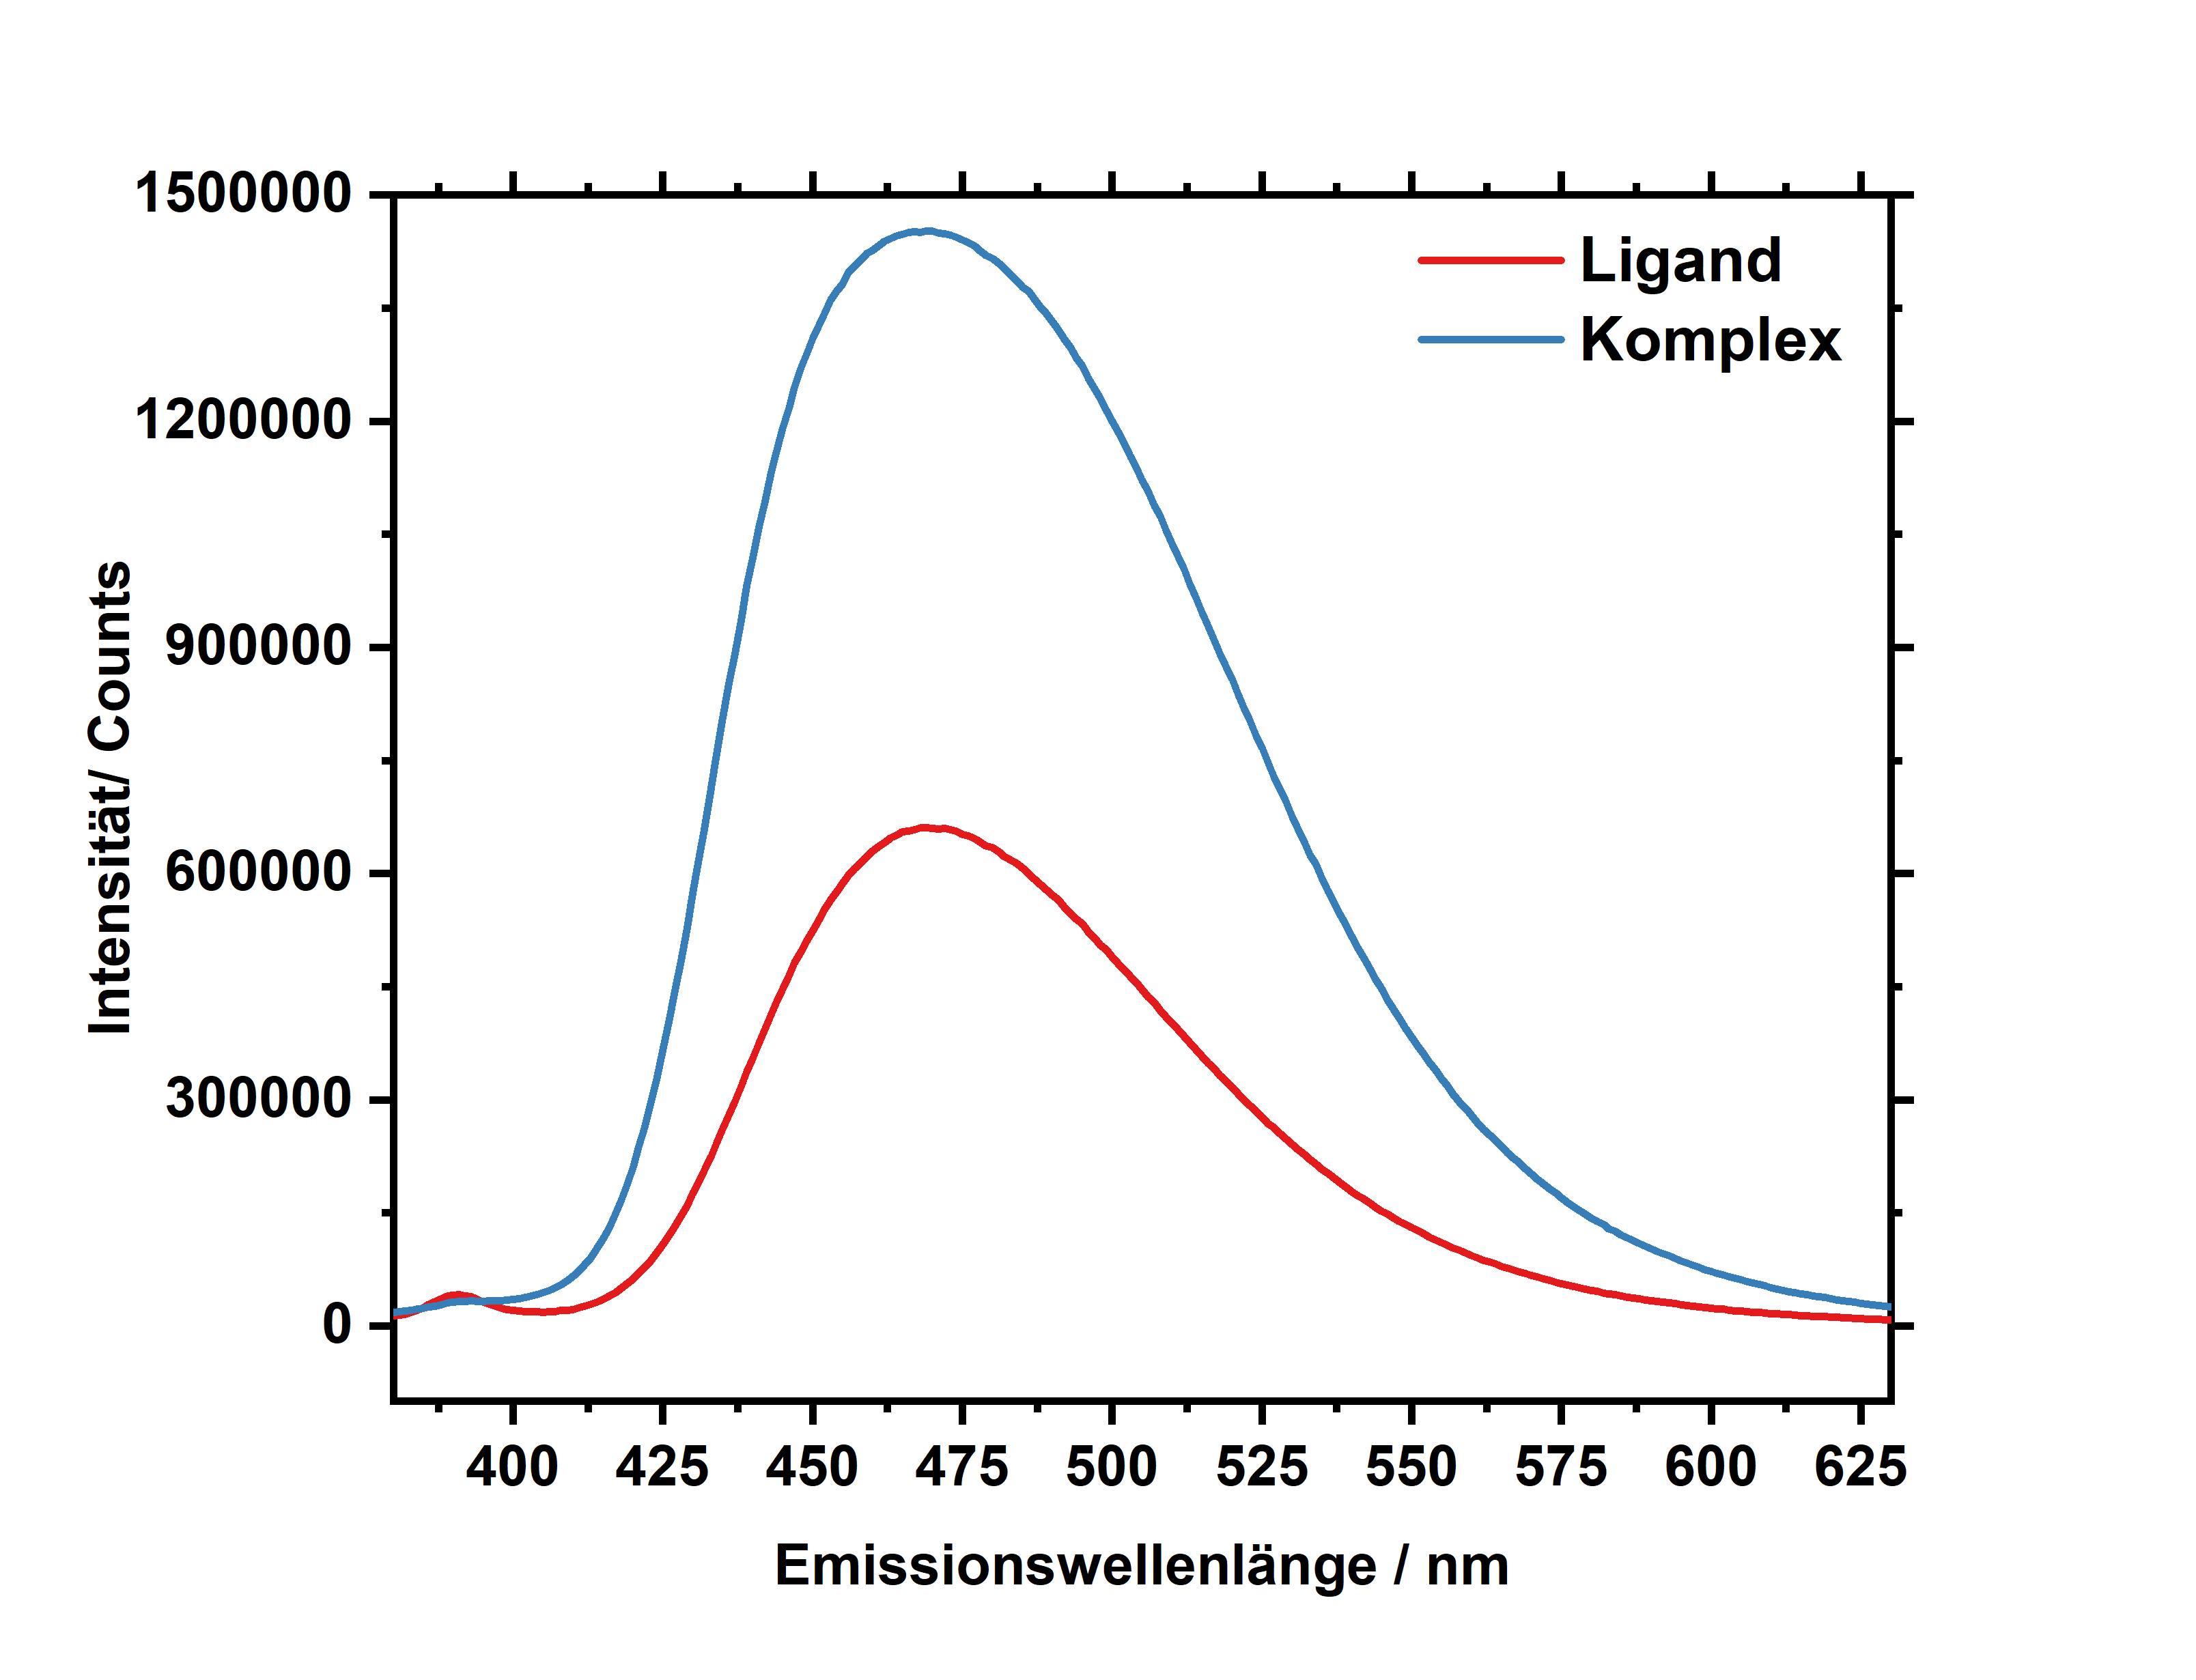
\includegraphics[width=0.8\textwidth]{FluoreszenzLigandKomplex.jpg}
			\textbf{\caption{\textnormal{Emissionsspektrum des Liganden (rot, c = 3,75 \textmu mol \ce{L^{-1}}) und des Komplexes (blau, c = 0,008 \textmu mol \ce{L^{-1}}) in Ethanol im Wellenlängenbereich von 290 - 480 nm.}}}
			\label{fig:FluoreszenzLigandKomplex}
		\end{figure}\\
	Ursache ist die Unterbindung von PET-Prozessen durch die Bindung der freien Elektronenpaare am Stickstoff sowie \\
	\ \\
	Keine Interaktion und der Hydroxygruppe, da keine Blau-Verschiebung des Maximums,
	
	\section{Immobilisierung}
	\subsection{Pyranin}
	Beim immobiliserten Pyranin wurden zunächst zwei Emissionsmaxima gemessen, wobei der Peak bei 515 nm nach einer Spülung des Chips mit Wasser verschwindet (\textbf{\autoref{fig:PyraninFlow}}).
		\begin{figure}[h!]
			\centering 
			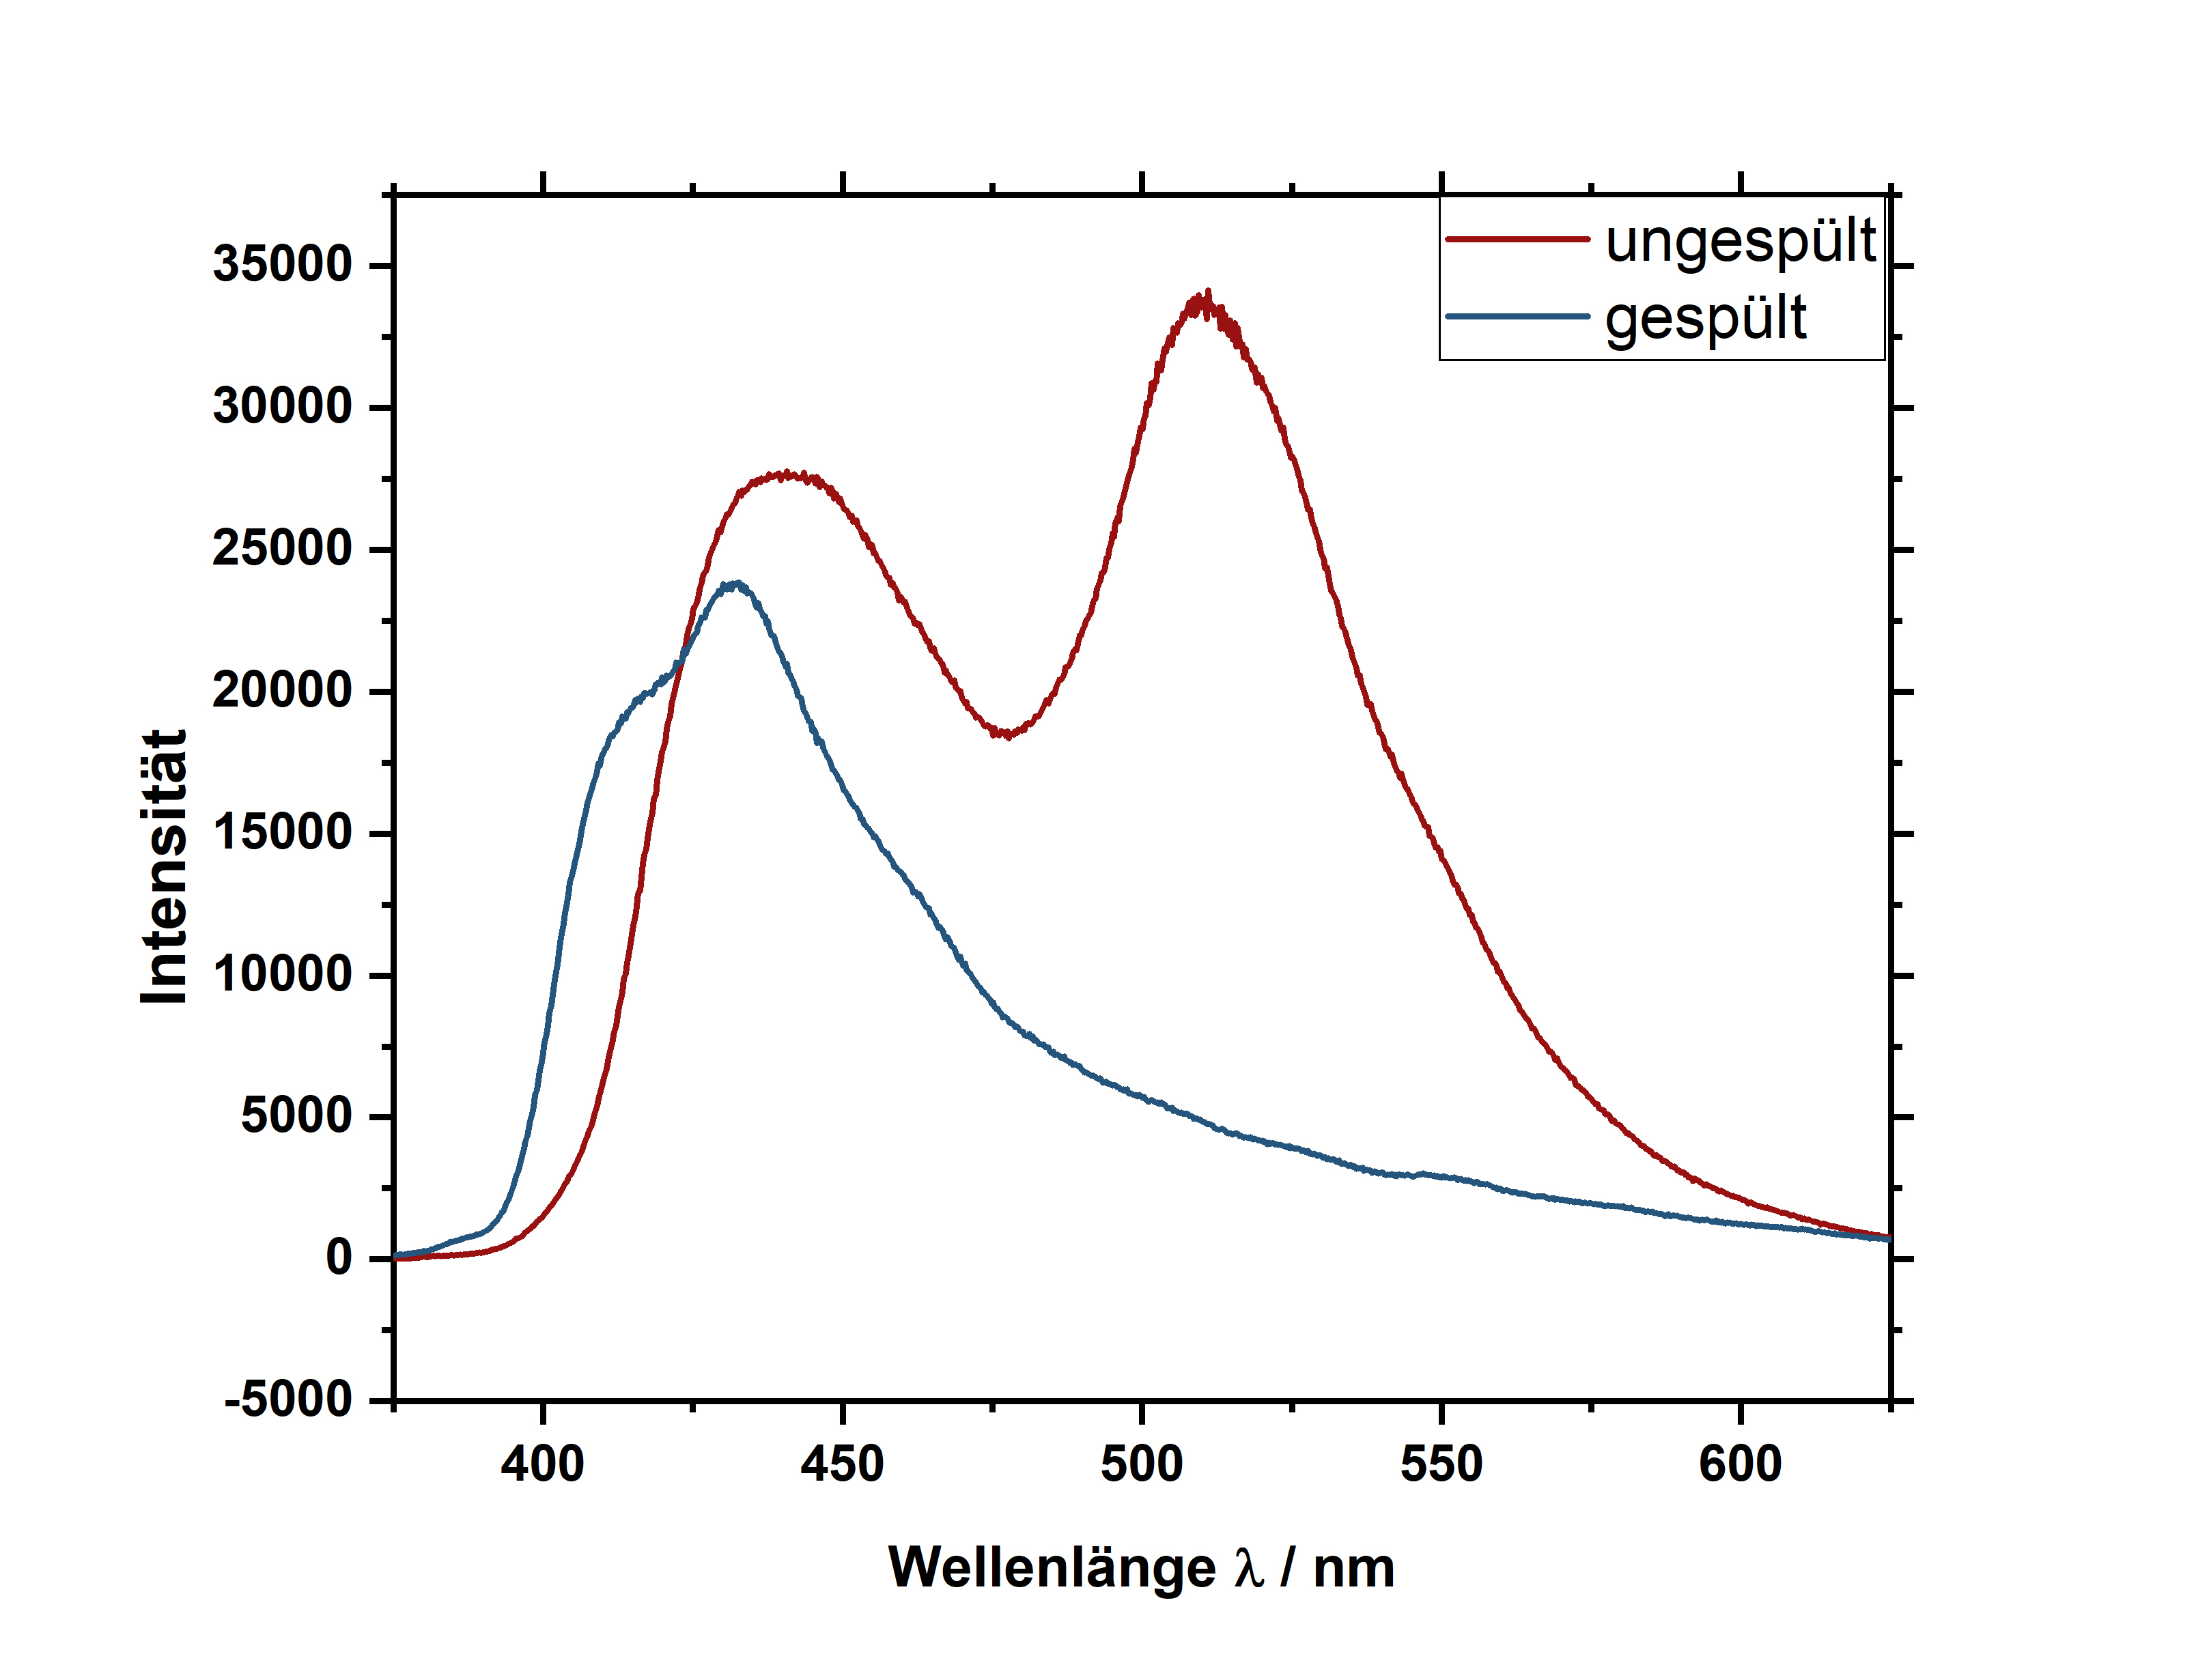
\includegraphics[width=0.8\textwidth]{FlowPyranin.jpg}
			\textbf{\caption{\textnormal{Fluoreszenzspektrumdes Pyranins in bei einer Anregungswellenlänge von}}}
			\label{fig:PyraninFlow}
		\end{figure}
	\textit{Kızıldereli et al} beobachtete, dass infolge einer C-O-Ether Bindung zwischen der Hydroxygruppe des Pyranins und dem terminalen C-Atoms des Acrylamids eine hypsochrome Verschiebung, von 515 nm zu 406 nm, im Emissionsspektrum des Pyranins auftritt. Gleichzeitig verursachen elektrostatische Wechselwirkungen zwischen den Sulfonsäuregruppen und den protonierten Amidgruppen der AAm-Ketten eine bathochrome Verschiebung des Peaks, von 406 zu 430 nm.\\
	\ \\
	Demnach können die beiden Maxima bei nm und nm im ungespülten Zustand auf gebundenes sowie und gebundenes Pyranin zurückgeführt werden. Diese Überlegung wird dadurch gestützt, dass der Peak des freien Pyranins bei 50 nm durch die Spülung des Chips mit Wasser verschwindet. Dies ist mit der sehr guten Wasserlöslichkeit des Pyranins (300 g/l) vereinbar. 
	\subsection{Ligand und Komplex}
	\section{Flowansatz}
	\subsection{Pyranin}
	\subsection{Ligand und Komplex}
	\chapter{Diskussion}
	Anhand der spektroskopischen Charakterisierung konnte gezeigt werden, dass Calixaren als fluoreszierender Chemosensor für \ce{Zn^{2+}}-Ionen eingesetzt werden kann. Die Selektivität des Liganden ist dabei Gegenstand weiterer Untersuchungen. Auch wurde die Abhängigkeit zwischen Konzentration der Zinklösung und der Fluoresznez nicht untersucht
	\chapter{Ausblick}
	\chapter{Experimentalteil}
	\chapter{Literaturverzeichnis}
\end{document}